\section{Zielsetzung}
    Es soll das Elastizitätsmodul verschiedener elastischer Stäbe untersucht werden und diese anschließend 
    mit Literaturwerten verglichen werden, um so das Metall zu bestimmen.
\section{Theorie}
\label{sec:theorie}
    Das Elastizitätsmodul $E$ beschreibt die Deformation eines Körpers unter der Einwirkung einer Normalspannung $\sigma$. Als Normalspannung wird dabei eine Kraft
    bezeichnet, welche senkrecht auf der Oberfläche steht. Über das Hook'sche Gesetz lässt sich ein Zusammenhang zwischen der Normalspannung $\sigma$ und
    der Deformation $\frac{\delta L}{L}$ herstellen:
    \begin{equation}
    \label{eqn:hook}
        \sigma = E \, \frac{\delta L}{L}.
    \end{equation}
  %Mit der Ausgangslänge $\delta x$ und dem Krümmungsradius $R$ und der Annahme, dass $\Delta x << \delta x$ ergibt sich für die Längenänderung:
  %  \begin{equation}
  %  \label{eqn:laenge}
  %      \Delta x = y \delta\phi = y \frac{\delta x} {R}
  %  \end{equation}
    Das Elastizitätsmodul eines elastischen Stabes kann durch Einspannen an einem beziehungsweise beiden Enden bestimmt werden.
    \subsection{Einseitige Einspannung}
    \begin{figure}
        \centering
        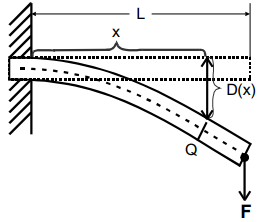
\includegraphics{content/einseitig.png}
        \caption{Schematische Darstellung der Durchbiegung eines elastisches Stabes bei einseitiger Einspannung. \cite[107]{V103}}
        \label{fig:einseitig}
    \end{figure}
        Beim einseitigen Einspannen, wie in \autoref{fig:einseitig} zu sehen, wird die Auslenkung $D(x)$ in Abhängigkeit von der Position $x$ am Stab gemessen.
        Durch Einwirken einer Kraft $F$ am Stab, entstehen zwei Drehmomente. Das äußere Drehmoment $M_F$ ist abhängig von der Kraft $F$ und dem Hebearm am Punkt $x$ und 
        ist daher 
        \begin{equation}
        \label{eqn:drehmomentA}
            M_F = F (L-x).
        \end{equation}
        Dieses muss entgegengesetzt gleich zum inneren Drehmoment $M_\sigma$, damit sich eine endliche Auslenkung $D(x)$ einstellt.
        Das innere Drehmoment ist definiert über den Abstand $y$ zwischen der neutralen Faser (die gestrichelte Linie in \autoref{fig:einseitig}), also die Fläche in der keine Spannungen
        auftreten, somit die Länge der Faser gleichbleibt, und dem Flächenelement $dQ$, sowie der angelegten Normalspannung $\sigma$. Durch Integration über die gesamte
        Querschnittsfläche $Q$ ergibt sich für das innere Drehmoment:
        \begin{equation}
        \label{eqn:drehmomentI} 
            M_\sigma = \int_Q y \, \sigma (y) \, \symup{d}Q.
        \end{equation}
        Eine Deformation stellt sich dann ein, wenn beide Drehmomente übereinstimmen, so dass sich beide Drehmomente gleichsetzen lassen.
        Über das Hook'sche Gesetz, Gleichung \eqref{eqn:hook}, und einiger differentialgeometrischer Zusammenhänge
        lässt sich die Normalspannung für eine Änderung der Länge des Stabes $\Delta x$ erechnen, zu:
        \begin{equation}
        \label{eqn:Normalspannung}
            \sigma(y) = E y \frac{\symup{d}^2 D}{\symup{d}x^2}.
        \end{equation}
        Hiermit ergibt sich für die gleichgesetzen Drehmomente der Zusammenhang
        \begin{equation}
        \label{eqn:gleichsetzung}
            E \frac{\symup{d}^2 D}{\symup{d}x^2} \int_Q y^2 \, \symup{d}q = F(L - x),
        \end{equation}
        wobei $D$ die Durchbiegung des Stabes ist.
        Mithilfe der Definition für das Flächenträgheitsmoment
        \begin{equation}
        \label{eqn:flaechentraegheitsmoment}
            I = \int_Q y^2 \, \symup{d}q
        \end{equation}
        und zweimaliger Integration nach $x$ ergibt sich die Durchbiegung für $0 \leq x \leq L$ zu
        \begin{equation}
        \label{eqn:durchbiegung1}
            D(x) = \frac{F}{2 E I} (L x^2 - \frac{1}{3} x^3).
        \end{equation}

    \subsection{Beidseitige Einspannung}
        \begin{figure}
            \centering
            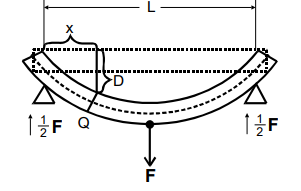
\includegraphics{content/beidseitig.png}
            \caption{Schematische Darstellung der Durchbiegung eines elastischen Stabes bei zweiseitiger Auflage. \cite[110]{V103}}
            \label{fig:beidseitig}
        \end{figure}
        Beim beidseitigem Einspannen eines elastischen Stabes, wie in \autoref{fig:beidseitig} zu sehen, wird das Gewicht in die Mitte des Stabes gehängt,
        wodurch sich die Kraft auf beide Häften des Stabes gleichmäßig verteilt.
        Somit gilt für die linke Hälfte ($0 \leq x \leq \frac{L}{2}$)
        \begin{equation}
        \label{eqn:mf1}
            M_\text{F1} = - \frac{F x } {2}
        \end{equation}
        und für die rechte Hälfte ($\frac{L}{2} \leq x \leq L $)    
        \begin{equation}
        \label{eqn:mf2}
            M_\text{F2} = - \frac {F}{2} (L - x).
        \end{equation}    
        Hieraus ließen sich wie zuvor bei der einseitigen Einspannung die Durchbiegungen $D$ erechnen.
        Hinzu kommt allerdings die Bedingung, dass die Biegekurve in der Mitte eine horizontale Tangente haben soll, sodass
        \begin{equation}
        \label{eqn:c1}
            C_1 = \frac{ F L^2} {16 E I}
        \end{equation}
        und 
        \begin{equation}
        \label{eqn:c2}
            C_2 = \frac{3 F L^2}{16 E I},
        \end{equation}
        womit sich die Durchbiegungen wie schon bei der einseitigen Einspannung ergeben, zu
        \begin{equation}
        \label{eqn:Durchbiegungbeidseitig1}
             D_1(x) =  \frac{F} {48 E I} (3L^2 x - 4 x^3)  
        \end{equation}
        für $0 \leq x \leq \frac{L}{2}$
        und für $\frac{L}{2} \leq x \leq L$
        \begin{equation}
        \label{eqn:Durchbiegungbeidseitig2}
           D_2(x) = \frac{F} {48 E I} (4 x^3 - 12 L x^2 + 9 L^2 x - L^3).
        \end{equation}   
